\section{Optimization in Real Life}

Now that we have seen the usage of differentiation as a rate of change measuring tool, we are now well-posed to formulate the usage of maxima and minima in real life, which is far more significant than the previous section in various areas of science and technology.

Now, we see how to solve geometrical and other optimization problems through examples.

\begin{enumerate}
    \item Let us say we have an x-y coordinate plane. And a point (a,b). What is the largest hypotenuse drawn through this point that will cut the axis and y-axis and create respective heights and bases?\\\\
        Let us draw a line that makes an angle $\alpha$ with the negative x-axis. 

        \begin{figure}[\ht]
            \centering
            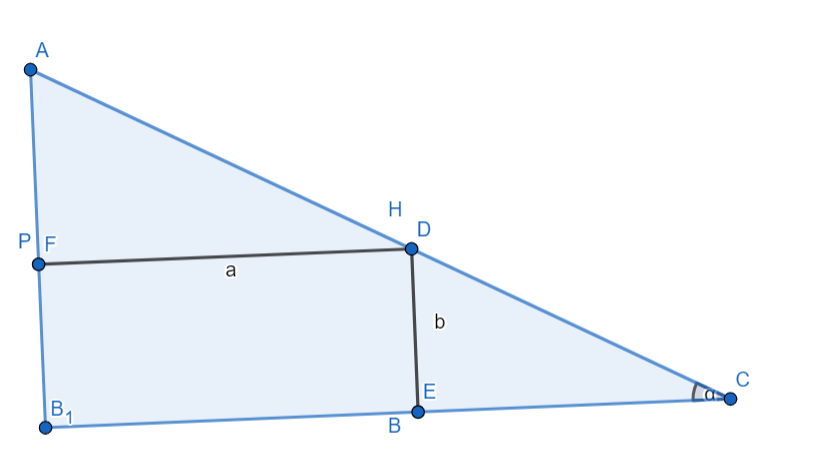
\includegraphics[width=0.5\linewidth]{sections_Calculus/Differentiation in Real Life/Opt_1.png}
            \caption{Triangle}
            \label{fig:enter-label}
        \end{figure}


        Now, the length of DA is $a\sec\alpha$, and the size of DC is $b\csc\alpha$.

        The total length of the hypotenuse is $a\sec\alpha+ b \csc\alpha$.

        This is a function of $\alpha$, which must be extremized. If we differentiate this function, then we get the derivative to be:

        $$a\sec\alpha \tan\alpha = b \csc\alpha \cot\alpha $$

        which in turn implies: $$\tan\alpha = \left( \frac{b}{a}\right)^{1/3}$$. If we put this into the original length equation, we get the lengths to be:

        $$l_{max}=\left(a^{2/3} + \b ^{2/3}\right)^{3/2}$$

        Now, intuitively this is the minimum length as if we make the angle $\alpha$ near to $\pi/2 $, or 0, the hypotenuse length goes to $\infty$
\end{enumerate}

